% @Author: AnthonyKenny98
% @Date:   2020-02-23 12:45:54
% @Last Modified by:   AnthonyKenny98
% @Last Modified time: 2020-03-01 09:17:29

\subsection{Background}
    
    The \ac{UAV} has been utilised in military applications extensively throughout the late 20th and early 21st century. However, over the last decade, their use in non-military uses, such as commerical, scientific, agricultural, and recreational, such that the number of civilian drones vastly outnumber military \ac{UAV}s.\todo{cite} Particularly in the commercial sector, such rapid growth in the number and range of applications means that autonomy is key for the profitable adoption of \ac{UAV}s. Such autonomy relies on efficient computation of motion planning algorithms. However, the implementation of these algorithms can be quite computationally expensive, and thus slow and/or detrimentally power consuming. As such, this thesis aims to design specialized hardware to more efficiently compute motion plans for autonomous drones.

    \subsubsection*{Robotics}
        For well over 2000 years, the concept of robotics, albeit not always with such a term, has fascinated humans. As early as the first century A.D., the Greek mathematician and engineer, Heron of Alexandria, described more than 100 different machines and automata in \textit{Pneumatica} and \textit{Automata} \cite{Alexandrinus}. In 1898, Nikola Tesla demonstrated the first radio-controlled vessel. Since then, the world has seen widespread application of robotics in manufacturing, mining, transport, exploration, and weaponry. For the last few decades, robots have operated in controlled, largely unchanging environments (e.g.\ an assembly line) where their environment and movements are largely known \textit{a priori}.
        \newline
        However, in recent years a new generation of autonomous robots has been developed for a wide range of real-world, complex applications. The increasing trend the use of autonomous robots is shown in Figure \ref{fig:useOfAutonomousRobots}. These new robots, unlike those traditional ones described above, are required to adapt to the changing environment in which they operate. As such, they must perform motion planning in real time.

        % @Author: AnthonyKenny98
% @Date:   2020-02-23 12:12:56
% @Last Modified by:   AnthonyKenny98
% @Last Modified time: 2020-02-23 13:56:51

\begin{figure}%[H]
\begin{center}
\missingfigure[figwidth=\linewidth]{Some sort of line/bar graph showing the increasing use of Autonomous robots over time. Need to find}
% 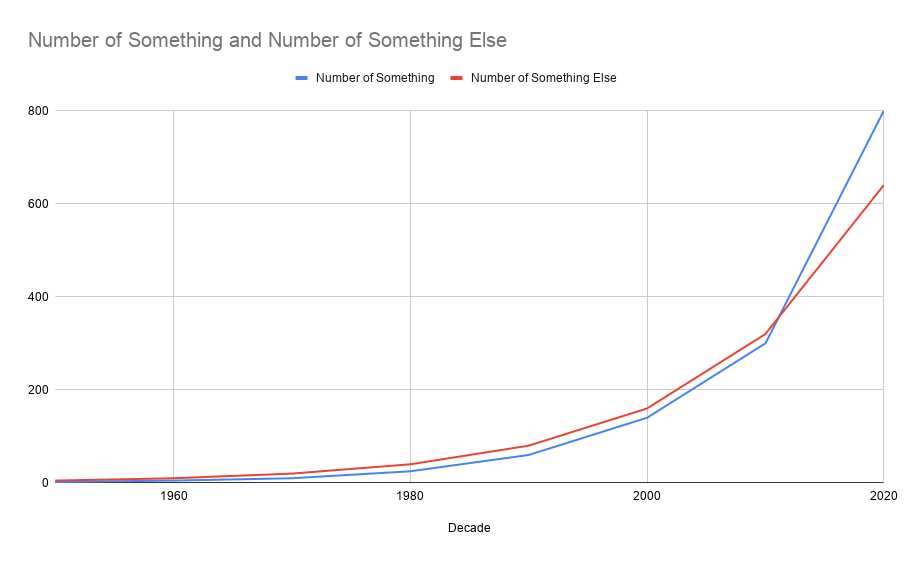
\includegraphics[width=0.8\linewidth]{img/sampleLineGraph.png}
\caption{The use of Autonomous Robots over time}
\label{fig:useOfAutonomousRobots}
\end{center}
\end{figure}

    \subsubsection*{Motion Planning}
        \todo[inline]{TODO: More of an introduction to motion planning.}
        
        Motion Planning refers to the problem of determining how a robot moves through a space to acheive a goal. Chapter \ref{chap:MotionPlanningInSoftware} provides a detailed explanation of motion planning and of \ac{RRT}, a commonly used motion planning algorithm.
        \newline
        On the algorithmic level, motion planning has been extensively studied and many solutions exist. However, current algorithms running on regular \ac{CPU}s are too slow to execute in real time for robots operating in complex environments. Simply solving this problem with more raw computing power, using energy hungry \ac{GPU}s may have merit in tethered robots. On the other hand, untethered applications, such as autonomous drones, where limiting power consumption is a primary concern, this strategy is infeasible.
        
    \subsubsection*{Something}
    \todo[inline, caption={Subsubsection for Problem Overview}]{Write something here about the current issue of slowness to transition into problem statement}

\newpage
\subsection{Problem Definition}

    \subsubsection*{Problem Statement}
    Motion planning algorithms implemented in software that runs on general purpose \ac{CPU}s cannot execute quickly enough for fully autonomous \ac{UAV}s to operate in high-complexity environments. The state-of-the-art strategy of using power-hungry \ac{GPU}s to accelerate the execution of these algorithms requires too much power to be cost-effective or feasible for \ac{UAV}s to sustain flight for useful periods of time. \todo[size=\small, inline, caption={Improve Problem Statement}]{Existing research into accelerating robotic motion planning is <reason for RISC-V, inaccessable?> and mainly focussed on tethered arm moveing robots.}

    \subsubsection*{End User}
    This thesis aims to provide developers of autonomous drones with specialized hardware for motion planning. Such developers have a need for computing hardware that executes motion planning algorithms faster and more power efficiently than existing methods. This thesis will provide a processor design that is synthesizable on an \ac{FPGA}, giving developers a processer for which a \ac{RTOS}, or bare metal code, can be deployed.
    \todo[inline]{Revise End User}